\documentclass{gh}

\usepackage{array}
\usepackage{longtable}
\usepackage{needspace}
\setlength{\LTpre}{4pt}

\tipodoc{Analisi dei requisiti}
\versione{0.0.3}
\datadoc{19/11/2026}
\redattori{D. Grosselle}
\verificatori{T. Caon}
\destinatari{Prof. T. Vardanega \\ Prof. R. Cardin \\ Halue Srl}

\begin{document}

\makeheader
% ==========================================
% REGISTRO DELLE MODIFICHE
% ==========================================
\noindent{\Large \textbf{Registro delle modifiche}}\\[0.5cm]

\renewcommand{\arraystretch}{1.3}
\noindent\begin{tabularx}{\textwidth}{|c|c|>{\raggedright\arraybackslash}p{2.8cm}|>{\raggedright\arraybackslash}p{2.8cm}|X|}
    \hline
    \textbf{Versione} & \textbf{Data} & \textbf{Autore} & \textbf{Verificatore} & \textbf{Dettaglio} \\
    \hline
    0.1.1 & 2026/11/22 & D. Grosselle & T. Caon & Casi d'uso UC1, UC2, UC3 e sottocasistiche \\
    \hline
    0.1.0 & 2026/11/22 & D. Grosselle & T. Caon & Stesura sezione 3.1, 3.2  \\
    \hline
    0.0.3 & 2026/11/19 & D. Grosselle & T. Caon & Stesura sezione Descrizione del prodotto  \\
    \hline
    0.0.2 & 2026/11/18 & D. Grosselle & T. Caon & Stesura sezione Introduzione \\
    \hline
    0.0.1 & 2026/11/7 & D. Grosselle & T. Caon & Struttura documento \\
    \hline
\end{tabularx}
\newpage

\tableofcontents
\newpage
\renewcommand{\arraystretch}{1.3}
\section{Introduzione}

\subsection{Scopo del documento}
Lo scopo del presente documento è di descrivere in modo dettagliato i casi d'uso e i requisiti del prodotto software associato al capitolato d'appalto \textbf{C8 - Sonar: Documentazione vivente di uno store Shopify} proposto dall'azienda Halue S.r.l. SB.\\ 
\\
L'analisi viene condotta a seguito di un'attenta disamina del capitolato e di un confronto continuo con la proponente attraverso i canali di comunicazione concordati.\\ 
Il documento si rivolge ai membri del gruppo \textit{Git Happens}, ai committenti e ai docenti di riferimento, fungendo da base per le successive fasi di progettazione, codifica e verifica.

\subsection{Glossario}
Per prevenire incomprensioni legate all'uso di termini tecnici o specifici del dominio, il gruppo ha redatto il \textit{Glossario}.\\
Ogni termine che assume un significato specifico all'interno del contesto di progetto viene contrassegnato nel testo da una lettera G posta a pedice. Tale marcatura indica che la definizione formale e condivisa del termine è consultabile all'interno del documento di glossario.

\subsection{Riferimenti}
\subsubsection{Riferimenti normativi}
\begin{itemize}
    \item \textit{Norme di Progetto}
    \item \textbf{Capitolato C8 - Sonar}: Documentazione vivente di uno store Shopify (Halue S.r.l. SB):\\
    \url{https://www.math.unipd.it/~tullio/IS-1/2026/Progetto/C8-Sonar.pdf}\\
    (Consultato: )
    \item \textbf{Regolamento del progetto didattico:} \\
    \url{https://www.math.unipd.it/~tullio/IS-1/2026/Dispense/PD1.pdf} (Consultato: );
    \item \textbf{Standard ISO/IEC 12207:1995:} \\
    \url{https://www.math.unipd.it/~tullio/IS-1/2009/Approfondimenti/ISO_12207-1995.pdf} (Consultato: ).
\end{itemize}

\subsubsection{Riferimenti informativi}
\begin{itemize}
    \item \textit{Glossario};
    \item \textbf{Slide del corso di Ingegneria del Software - Ciclo di vita del software:} \\
    \url{https://www.math.unipd.it/~tullio/IS-1/2026/Dispense/T02.pdf} (Consultato: );
    \item \textbf{Slide del corso di Ingegneria del Software - Gestione di progetto:} \\
    \url{https://www.math.unipd.it/~tullio/IS-1/2026/Dispense/T04.pdf} (Consultato: );
    \item \textbf{Documentazione Shopify API \& Developer Platform:} \\
    \url{https://shopify.dev/docs} (Consultato: );
    \item \textbf{Documentazione Next.js:} \\
    \url{https://nextjs.org/docs} (Consultato: ).
\end{itemize}
\section{Descrizione del prodotto}

\subsection{Obiettivi}
Il progetto \textbf{Sonar} nasce dall'esigenza dell'azienda proponente \textit{Halue S.r.l. Società Benefit} di realizzare una piattaforma web per la generazione automatica e ripetibile della documentazione vivente di store \textit{Shopify} di dimensioni \textit{enterprise}. \\
Nel corso del loro ciclo di vita, gli store di grandi dimensioni tendono a trasformarsi in sistemi stratificati, accumulando applicazioni di terze parti, \textit{webhook}, definizioni di \textit{metafield}, \textit{metaobject} e frammenti di codice di tema di cui si perde progressivamente traccia. \\
\\
Il principio cardine del sistema è che l'unica documentazione affidabile nel tempo non può dipendere dalla disciplina manuale degli sviluppatori, bensì deve essere ricostruita automaticamente dal sistema stesso a ogni scansione. L'obiettivo di \textbf{Sonar} non si limita a fornire un inventario statico di ciò che esiste nello store, ma mira a ricostruire l'intera rete delle dipendenze reciproche per rispondere a quesiti architetturali critici (es. valutare l'impatto della rimozione di una risorsa) e identificare componenti orfani o codice morto.

\subsection{Funzionalità}
L'architettura funzionale di \textbf{Sonar} si articola in cinque fasi sequenziali, progettate per mantenere una netta separazione delle responsabilità (\textit{separation of concerns}):
\begin{enumerate}
    \item \textbf{Acquisizione (Scansione)}\\
    Esecuzione di interrogazioni durevoli e resilienti verso le API di Shopify (GraphQL e REST) e lettura dei file del tema, finalizzate a produrre uno \textit{snapshot}, ovvero una fotografia immutabile e datata dello stato dello store. \\
    Per superare i limiti strutturali delle API di Shopify su store di grandi dimensioni, il processo gestisce nativamente:
    \begin{itemize}
        \item \textbf{Paginazione tramite cursori:} per l'estrazione incrementale di elenchi molto estesi senza superare i limiti di \textit{rate limiting};
        \item \textbf{Triangolazione delle fonti:} poiché alcune entità non sono visibili da un unico endpoint (ad esempio, webhook registrati da app terze), il sistema incrocia fonti eterogenee per massimizzare la copertura dell'inventario;
        \item \textbf{Telemetria interna:} registrazione puntuale delle risorse consumate per ogni singola scansione (chiamate API, passi di workflow, token LLM).
    \end{itemize}
    \item \textbf{Normalizzazione e modello a grafo} \\
    Trasformazione dei dati grezzi raccolti in un modello a grafo unificato. I \textbf{nodi} rappresentano le entità strutturali dello store (applicazioni, webhook, definizioni di metafield, file di tema, funzioni, canali di vendita), mentre gli \textbf{archi} codificano le dipendenze dirette e indirette tra di essi. \\
    Ogni arco è corredato dalla fonte dell'evidenza e da un \textbf{livello di confidenza} esplicito (\textit{accertato}, \textit{probabile} o \textit{ipotizzato});
    \item \textbf{Analisi statica del codice del tema}\\
    Ispezione isolata e sicura dei file del tema (in particolare template, sezioni e snippet scritti in linguaggio \textit{Liquid}) volta a rilevare i riferimenti ai metafield e a ricostruire il grafo di inclusione tra i file;
    \item \textbf{Rilevamento degli orfani e del codice morto}\\
    Applicazione di un motore di regole estensibile sul grafo normalizzato e sui risultati dell'analisi statica per individuare entità scollegate, definizioni di metafield mai referenziate né popolate, file di tema non inclusi e configurazioni obsolete;
    \item \textbf{Visualizzazione ed esportazione}\\
    Presentazione dei risultati tramite un'interfaccia web interattiva che consente di esplorare l'inventario, navigare visivamente il grafo delle dipendenze, filtrare le anomalie per livello di confidenza ed esportare la documentazione generata.
\end{enumerate}

\subsubsection{Vincoli e limiti di dominio}
Al fine di delimitare con precisione i confini operativi del sistema ed evitare ambiguità progettuali, sono stabiliti i seguenti vincoli di esclusione:
\begin{itemize}
    \item \textbf{Operatività strettamente in sola lettura}\\
    Sonar non apporta alcuna modifica agli store analizzati: non disinstalla applicazioni, non rimuove metafield, non altera il codice del tema. Il sistema si limita a segnalare le anomalie e a produrre istruzioni operative per eventuali interventi manuali da parte dei tecnici, richiedendo esclusivamente permessi (\textit{scope}) di sola lettura;
    \item \textbf{Assenza di monitoraggio in tempo reale}\\
    L'acquisizione dello stato dello store avviene unicamente tramite scansioni avviate manualmente su richiesta o secondo pianificazione periodica, senza flussi continui in tempo reale;
    \item \textbf{Esclusione dell'analisi prestazionale}\\
    Il sistema non rileva né valuta metriche di performance dello store o dello storefront;
    \item \textbf{Nessuna gestione dei dati di business}\\
    Entità commerciali quali prodotti, ordini e anagrafiche clienti non rientrano nel dominio applicativo di Sonar. Tali risorse vengono consultate unicamente in forma aggregata e statistica come evidenza per verificare l'effettivo utilizzo dei metafield configurati.
\end{itemize}

\subsection{Caratteristiche dell'utente}
Il prodotto si rivolge a figure professionali con competenze tecniche che operano nella gestione, manutenzione ed evoluzione di ecosistemi e-commerce complessi, quali:
\begin{itemize}
    \item \textbf{Sviluppatori Shopify e Full-Stack:} incaricati di intervenire sul codice del tema, integrare nuove applicazioni o effettuare attività di refactoring e pulizia del debito tecnico;
    \item \textbf{Architetti Software e Tech Lead:} responsabili della supervisione architetturale dello store, dell'audit tecnico e della valutazione dei rischi prima di rilasci evolutivi o migrazioni;
    \item \textbf{Project Manager tecnici e Solution Architect:} interessati a ottenere rapidamente una mappatura oggettiva e documentata dello stato di salute di uno store in fase di presa in carico (\textit{onboarding}) o consulenza.
\end{itemize}
Tali utenti possiedono familiarità con le architetture web e con i concetti base di Shopify, ma necessitano di uno strumento automatizzato che riduca i tempi di ispezione manuale e prevenga errori derivanti da dipendenze nascoste.

\subsection{Tecnologie}
In conformità con i vincoli architetturali imposti dal capitolato d'appalto, l'ecosistema tecnologico del prodotto si fonda sulle seguenti componenti:
\begin{itemize}
    \item \textbf{Framework applicativo:} \textbf{Next.js} per lo sviluppo dell'interfaccia web e delle API interne;
    \item \textbf{Infrastruttura di esecuzione e orchestrazione:} ecosistema \textbf{Vercel}, articolato in:
    \begin{itemize}
        \item \textit{Vercel Workflows} e \textit{Queues} per garantire l'esecuzione durevole delle scansioni e la ripresa automatica in caso di rate limiting o interruzioni;
        \item \textit{Vercel Sandbox} per l'esecuzione isolata e sicura dell'analisi statica sui file del tema;
        \item \textit{Vercel Blob} (per l'archiviazione degli snapshot grezzi).
    \end{itemize}
    \item \textbf{Persistenza e sicurezza dei dati:} \textbf{Supabase} (PostgreSQL) per la memorizzazione relazionale delle entità, del grafo delle dipendenze e delle metriche di scansione, protetto tramite politiche di \textit{Row Level Security (RLS)} per garantire l'isolamento multi-tenant dei dati;
    \item \textbf{Autenticazione verso Shopify:} gestione sicura delle credenziali di connessione agli store, inclusa l'archiviazione cifrata e il rinnovo automatico dei token di accesso generati tramite flusso \textit{client credentials}, soggetti a scadenza ogni 24 ore secondo le policy Shopify introdotte dal 2026.
\end{itemize}

\section{Casi d'uso}

\subsection{Introduzione}
Questa sezione illustra i casi d'uso delineati a seguito dell'analisi del capitolato d'appalto, del confronto continuo con l'azienda proponente \textit{Halue S.r.l. SB} e delle attività di analisi interne condotte dal gruppo \textit{Git Happens}. \\
\\
Ciascun caso d'uso fornisce una descrizione dettagliata delle funzionalità del sistema dal punto di vista degli utenti e delle entità esterne, illustrando come la piattaforma risponde a determinate azioni o scenari operativi. \\
In conformità con quanto stabilito nel documento \textit{Norme di Progetto} (TODO: inserire sezione una volta scritta), ogni caso d'uso è identificato da un codice univoco secondo la sintassi \texttt{UC[Numero caso d'uso].[Numero sottocaso d'uso] - [Titolo]} ed è accompagnato dai diagrammi UML di riferimento e da una scheda testuale strutturata nei seguenti campi:
\begin{itemize}
    \item \textbf{Identificativo e Titolo:} codice univoco e descrizione sintetica dell'obiettivo funzionale;
    \item \textbf{Attore principale:} entità esterna che avvia e guida attivamente l'interazione con il sistema per soddisfare una propria necessità;
    \item \textbf{Descrizione:} sintesi esplicativa della funzionalità modellata;
    \item \textbf{Precondizioni:} stato in cui deve trovarsi il sistema affinché l'interazione possa avere inizio;
    \item \textbf{Postcondizioni:} stato risultante del sistema al termine della corretta esecuzione dello scenario principale;
    \item \textbf{Scenario principale:} sequenza ordinata e numerata delle azioni e risposte che conducono al raggiungimento delle postcondizioni;
    \item \textbf{Estensioni:} eventuali flussi alternativi o di gestione degli errori che deviano dallo scenario principale al verificarsi di specifiche condizioni;
    \item \textbf{User story associata:} formulazione sintetica della funzionalità dal punto di vista dell'utente, volta a chiarirne il contesto e il valore operativo.
\end{itemize}

\subsection{Attori}
Gli attori rappresentano le entità esterne (utenti umani, sistemi software o componenti temporali) che interagiscono con il sistema \textbf{Sonar}.\\
\\
Dall'analisi del dominio applicativo sono stati individuati i seguenti attori:
\begin{itemize}
    \item \textbf{Utente non autenticato:} soggetto che accede all'interfaccia web di \textbf{Sonar} senza disporre ancora di una sessione attiva, la cui interazione è limitata alla procedura di autenticazione tramite provider esterno;
    \item \textbf{Utente autenticato:} utente tecnico (sviluppatore, architetto software o \textit{Tech Lead}) che ha completato con successo l'accesso ed è associato a una specifica organizzazione (\textit{tenant}). \\
    È abilitato a registrare e gestire gli store Shopify della propria organizzazione, avviare scansioni manuali, pianificare scansioni ricorrenti, esplorare lo stato degli snapshot e navigare il grafo delle dipendenze;
    \item \textbf{Temporizzatore (Scheduler):} entità temporale di sistema che avvia automaticamente, al raggiungimento delle scadenze pianificate, i flussi di lavoro durevoli per l'esecuzione delle scansioni periodiche sugli store configurati.
\end{itemize}

\subsection{Casi d'uso}

\subsubsection{UC1 - Autenticazione}
\begin{figure}[htbp]
    \centering
    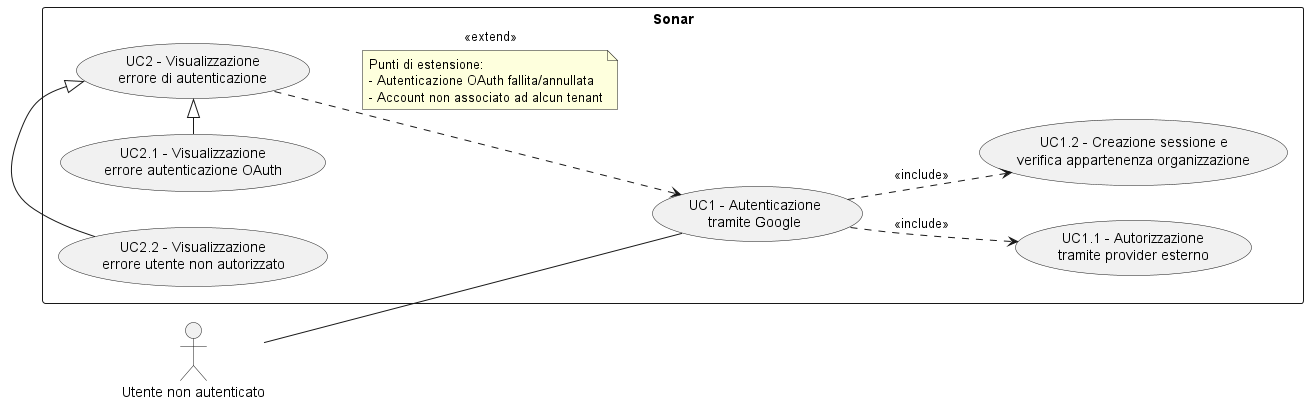
\includegraphics[width=0.9\textwidth]{assets/uc1.png}
    \caption{UC1 - Autenticazione}
    \label{fig:uc1}
\end{figure}

\begin{itemize}
    \item \textbf{Attore principale:} Utente non autenticato;
    \item \textbf{Descrizione:} L'utente effettua l'accesso alla piattaforma \textbf{Sonar} utilizzando il proprio account Google tramite il servizio di autenticazione integrato;
    \item \textbf{Precondizioni:} Il sistema è operativo e raggiungibile; l'utente non dispone di una sessione attiva;
    \item \textbf{Postcondizioni:} L'utente è autenticato, associato alla propria organizzazione (\textit{tenant}) e visualizza la dashboard degli store di competenza;
    \item \textbf{Scenario principale:}
    \begin{enumerate}
        \item L'utente accede alla schermata di login del sistema (direttamente oppure a seguito di reindirizzamento automatico da una pagina protetta);
        \item L'utente avvia la procedura selezionando l'opzione di accesso tramite Google;
        \item L'utente completa la verifica dell'identità presso il provider esterno (\textbf{include UC1.1});
        \item Il sistema istanzia la sessione di lavoro e verifica l'appartenenza dell'utente a un'organizzazione (\textbf{include UC1.2});
        \item Il sistema reindirizza l'utente alla dashboard principale mostrando esclusivamente gli store associati al suo \textit{tenant}.
    \end{enumerate}
    \item \textbf{Estensioni:}
    \begin{itemize}
        \item Autenticazione annullata dall'utente o rifiutata dal provider Google: il flusso è esteso da \textbf{UC2.1 - Visualizzazione errore autenticazione OAuth};
        \item Account Google valido ma non associato ad alcuna organizzazione censita: il flusso è esteso da \textbf{UC2.2 - Visualizzazione errore utente non autorizzato}.
    \end{itemize}
    \item \textbf{User story associata:} Come utente non autenticato voglio accedere al sistema tramite il mio account Google per consultare e gestire in sicurezza gli store della mia organizzazione.
\end{itemize}

\subsubsection{UC1.1 - Autorizzazione tramite provider esterno}
\begin{itemize}
    \item \textbf{Attore principale:} Utente non autenticato;
    \item \textbf{Descrizione:} L'utente interagisce con la schermata di consenso del provider OAuth (Google) per autorizzare l'identificazione verso \textbf{Sonar};
    \item \textbf{Precondizioni:} L'utente ha avviato \textbf{UC1} selezionando l'accesso tramite Google;
    \item \textbf{Postcondizioni:} Il provider esterno conferma l'identità dell'utente e restituisce al sistema un codice di autorizzazione valido;
    \item \textbf{Scenario principale:}
    \begin{enumerate}
        \item Il sistema reindirizza il browser dell'utente verso la pagina di autenticazione del provider Google;
        \item L'utente seleziona il proprio account Google e concede il consenso all'accesso;
        \item Il provider reindirizza l'utente all'endpoint di callback del sistema fornendo il token di autorizzazione.
    \end{enumerate}
    \item \textbf{User story associata:} Come utente non autenticato voglio autorizzare Sonar tramite il mio account Google senza dover creare nuove credenziali dedicate.
\end{itemize}

\subsubsection{UC1.2 - Creazione sessione e verifica appartenenza organizzazione}
\begin{itemize}
    \item \textbf{Attore principale:} Utente non autenticato;
    \item \textbf{Descrizione:} Il sistema valida l'identità ricevuta, avvia la sessione applicativa e associa l'utente al rispettivo \textit{tenant};
    \item \textbf{Precondizioni:} Il flusso \textbf{UC1.1} si è concluso con successo;
    \item \textbf{Postcondizioni:} La sessione dell'utente è attiva e il contesto organizzativo è stato determinato;
    \item \textbf{Scenario principale:}
    \begin{enumerate}
        \item Il sistema verifica la validità del token ricevuto tramite \textit{Supabase Auth};
        \item Il sistema interroga la base di dati per individuare l'organizzazione (\textit{tenant}) associata all'identità dell'utente;
        \item Il sistema genera i cookie/token di sessione sicuri lato client.
    \end{enumerate}
    \item \textbf{User story associata:} Come utente voglio che il sistema riconosca automaticamente la mia organizzazione al termine dell'accesso per operare nel corretto ambiente di lavoro.
\end{itemize}

\subsubsection{UC2 - Visualizzazione errore di autenticazione}
\begin{itemize}
    \item \textbf{Attore principale:} Utente non autenticato;
    \item \textbf{Descrizione:} Il sistema gestisce il mancato completamento della procedura di accesso notificando l'anomalia all'utente;
    \item \textbf{Precondizioni:} È stato avviato \textbf{UC1}, ma si è verificata un'anomalia durante l'autorizzazione o la verifica organizzativa;
    \item \textbf{Postcondizioni:} Nessuna sessione viene attivata e l'utente visualizza un messaggio diagnostico nella schermata di login;
    \item \textbf{Scenario principale:}
    \begin{enumerate}
        \item Il sistema intercetta l'interruzione o il fallimento della procedura di accesso;
        \item Il sistema impedisce l'accesso alle risorse protette e visualizza un messaggio esplicativo privo di dettagli tecnici sensibili.
    \end{enumerate}
    \item \textbf{User story associata:} Come utente non autenticato voglio essere informato in modo chiaro qualora il tentativo di accesso non vada a buon fine.
\end{itemize}

\subsubsection{UC2.1 - Visualizzazione errore autenticazione OAuth}
\begin{itemize}
    \item \textbf{Attore principale:} Utente non autenticato;
    \item \textbf{Descrizione:} Specializzazione di \textbf{UC2} relativa al rifiuto, all'annullamento o al fallimento tecnico del flusso di autenticazione presso Google;
    \item \textbf{Precondizioni:} Durante \textbf{UC1.1} l'utente ha annullato il consenso oppure il provider ha restituito un errore di autenticazione;
    \item \textbf{Postcondizioni:} L'utente viene riportato alla pagina di login con un avviso che invita a ripetere l'accesso;
    \item \textbf{Scenario principale:}
    \begin{enumerate}
        \item Il sistema rileva l'assenza di un token valido o un codice di errore nel callback OAuth;
        \item Il sistema mostra un messaggio che notifica il mancato completamento dell'autenticazione con Google.
    \end{enumerate}
    \item \textbf{User story associata:} Come utente non autenticato voglio sapere se l'accesso con Google è stato annullato o non è riuscito per poter riprovare.
\end{itemize}

\subsubsection{UC2.2 - Visualizzazione errore utente non autorizzato}
\begin{itemize}
    \item \textbf{Attore principale:} Utente non autenticato;
    \item \textbf{Descrizione:} Specializzazione di \textbf{UC2} relativa al caso in cui l'account Google sia valido, ma non risulti censito o associato ad alcuna organizzazione in \textbf{Sonar};
    \item \textbf{Precondizioni:} Il flusso \textbf{UC1.1} ha avuto esito positivo, ma durante \textbf{UC1.2} non viene trovata alcuna associazione a un \textit{tenant};
    \item \textbf{Postcondizioni:} L'eventuale sessione temporanea viene invalidata e l'utente visualizza un messaggio di accesso negato;
    \item \textbf{Scenario principale:}
    \begin{enumerate}
        \item Il sistema rileva che l'utente autenticato non appartiene ad alcun \textit{tenant} attivo;
        \item Il sistema revoca la sessione appena creata e reindirizza alla schermata di login;
        \item Il sistema visualizza un messaggio che informa l'utente che il proprio account non è abilitato ad accedere alla piattaforma.
    \end{enumerate}
    \item \textbf{User story associata:} Come utente non autorizzato voglio ricevere un avviso esplicito se il mio account Google non è associato ad alcuna organizzazione abilitata.
\end{itemize}

\subsubsection{UC3 - Disconnessione dal sistema (Logout)}

\begin{figure}[htbp]
    \centering
    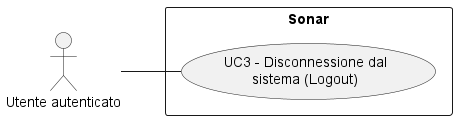
\includegraphics[width=0.9\textwidth]{assets/uc3.png}
    \caption{UC3 - Disconnessione}
    \label{fig:uc3}
\end{figure}

\begin{itemize}
    \item \textbf{Attore principale:} Utente autenticato;
    \item \textbf{Descrizione:} L'utente termina volontariamente la propria sessione di lavoro attiva all'interno della piattaforma \textbf{Sonar};
    \item \textbf{Precondizioni:} Il sistema è operativo e l'utente dispone di una sessione autenticata attiva;
    \item \textbf{Postcondizioni:} La sessione applicativa viene invalidata, i token di autenticazione lato client vengono revocati e l'utente viene reindirizzato alla schermata di login;
    \item \textbf{Scenario principale:}
    \begin{enumerate}
        \item L'utente seleziona il comando di disconnessione (\textit{logout}) dall'interfaccia web del sistema;
        \item Il sistema termina la sessione attiva tramite \textit{Supabase Auth} e rimuove i token/cookie di sessione lato client;
        \item Il sistema reindirizza l'utente alla pagina di autenticazione impedendo ulteriori accessi alle risorse protette.
    \end{enumerate}
    \item \textbf{User story associata:} Come utente autenticato voglio poter effettuare il logout per chiudere in sicurezza la mia sessione di lavoro.
\end{itemize}
\section{Requisiti}

\subsection{Requisiti funzionali}
\subsubsection{Requisiti funzionali obbligatori}
\subsubsection{Requisiti funzionali desiderabili}
\subsubsection{Requisiti funzionali opzionali}

\subsection{Requisiti qualitativi}
\subsubsection{Requisiti qualitativi obbligatori}

\subsection{Requisiti di vincolo}
\subsubsection{Requisiti di vincolo obbligatori}

\subsection{Requisiti prestazionali}

\subsection{Tracciamento}

\subsection{Riepilogo}


\end{document}
